\chapter{Introducción específica} % Main chapter title

\label{Chapter2}

%----------------------------------------------------------------------------------------
%	SECTION 1
%----------------------------------------------------------------------------------------
En este capítulo se introduce la terminología de la red de comunicaciones del tren y del sistema de información visual al pasajero. Se presenta una descripción de la arquitectura del sistema y de sus módulos principales. También se introduce el sistema de carteles led que presentan información al pasajeros, en particular en los coches de las formaciones ferroviarias de Trenes Argentinos.\\



\section{Trenes: Red de comunicación TCN}

La red de comunicaciones del tren (TCN) presenta una arquitectura de buses jerárquicos de dos niveles que se pueden identificar en la figura 1: el bus de datos WTB y el MVB\cite{IEC-61375-1999}. El WTB se encarga de las comunicaciones entre coches a través de nodos con redundancia física, mientras que al bus MVB se conectan los dispositivos de cada coche. Algunos de estos dispositivos son el control de puertas (DOORL/R), el aire acondicionado (HVAC), el sistema de tracción (VVVF), el sistema de control de frenos (BCU), entre otros. El mapa de recorrido y los carteles LED en conjunto con otros dispositivos como los parlantes y las cámaras de video (CCTV) forman un sistema denominado Sistema de información al pasajero (PIDS).



\begin{figure}[ht]
	\centering
	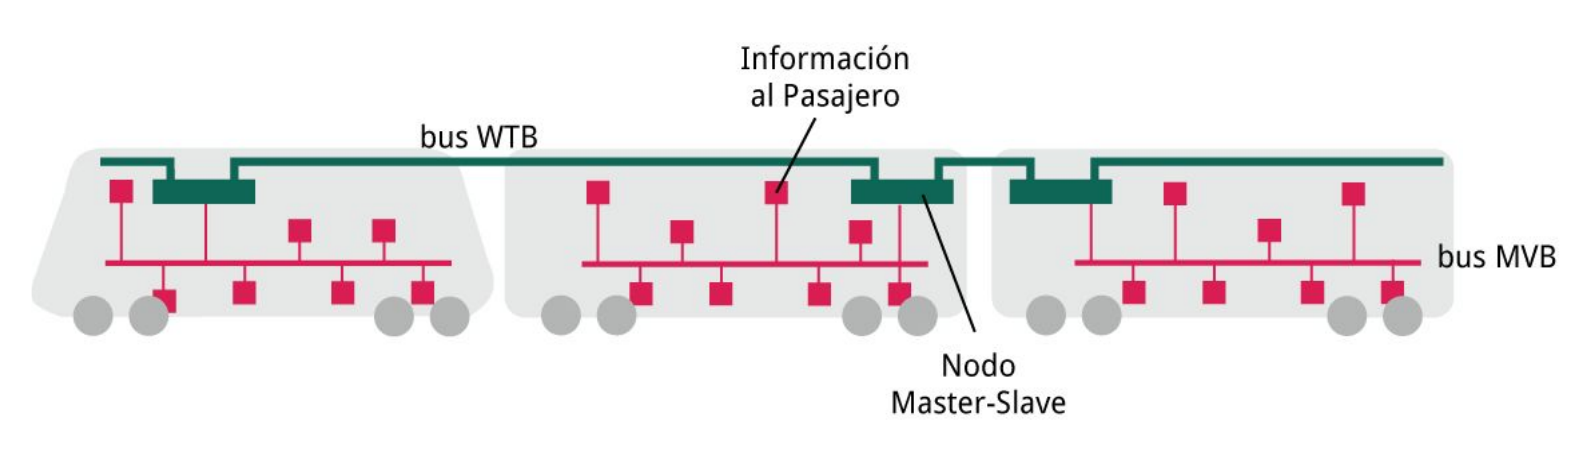
\includegraphics[width=1\textwidth]{./Figures/diagramaRedTCN.png}
	\caption{}
	\label{fig:redTCN}
\end{figure}


\begin{figure}[ht]
	\centering
	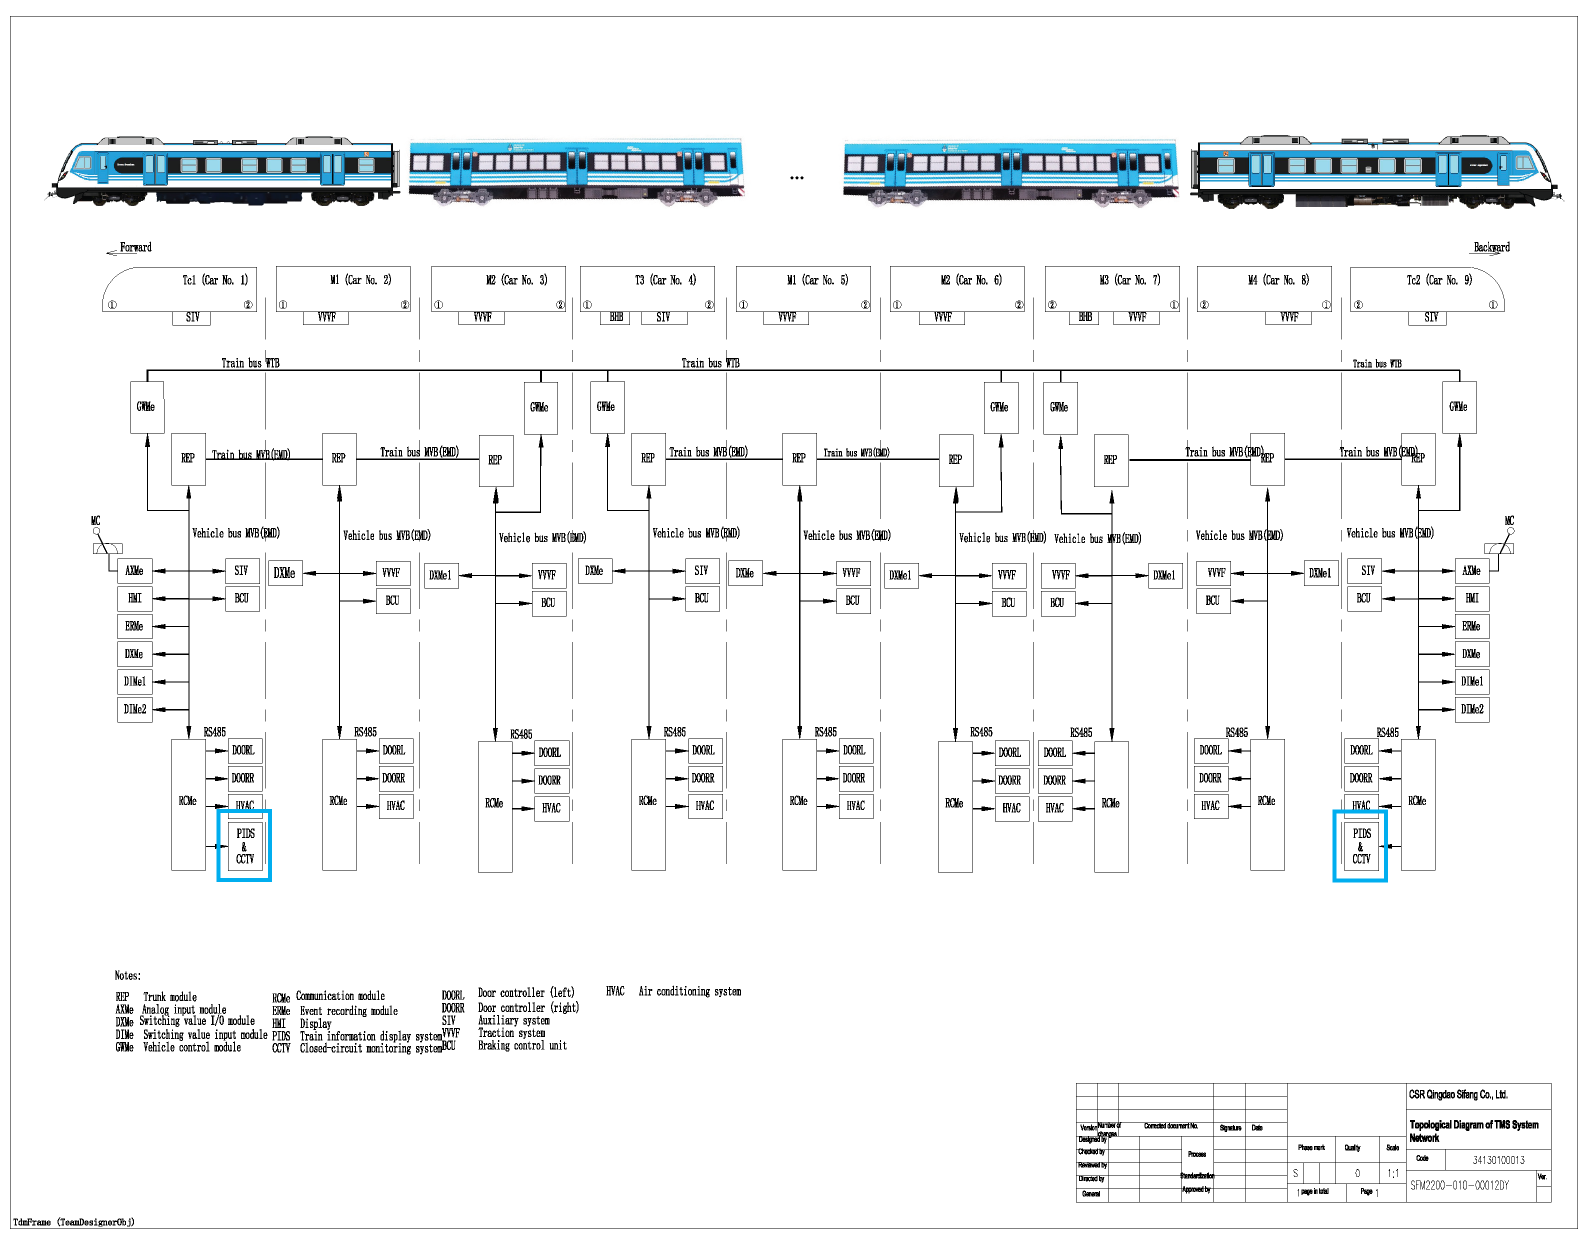
\includegraphics[width=1\textwidth]{./Figures/diagramaTrenesArgentinosTCN.png}
	\caption{}
	\label{fig:sofseTCN}
\end{figure}


\begin{figure}[ht]
	\centering
	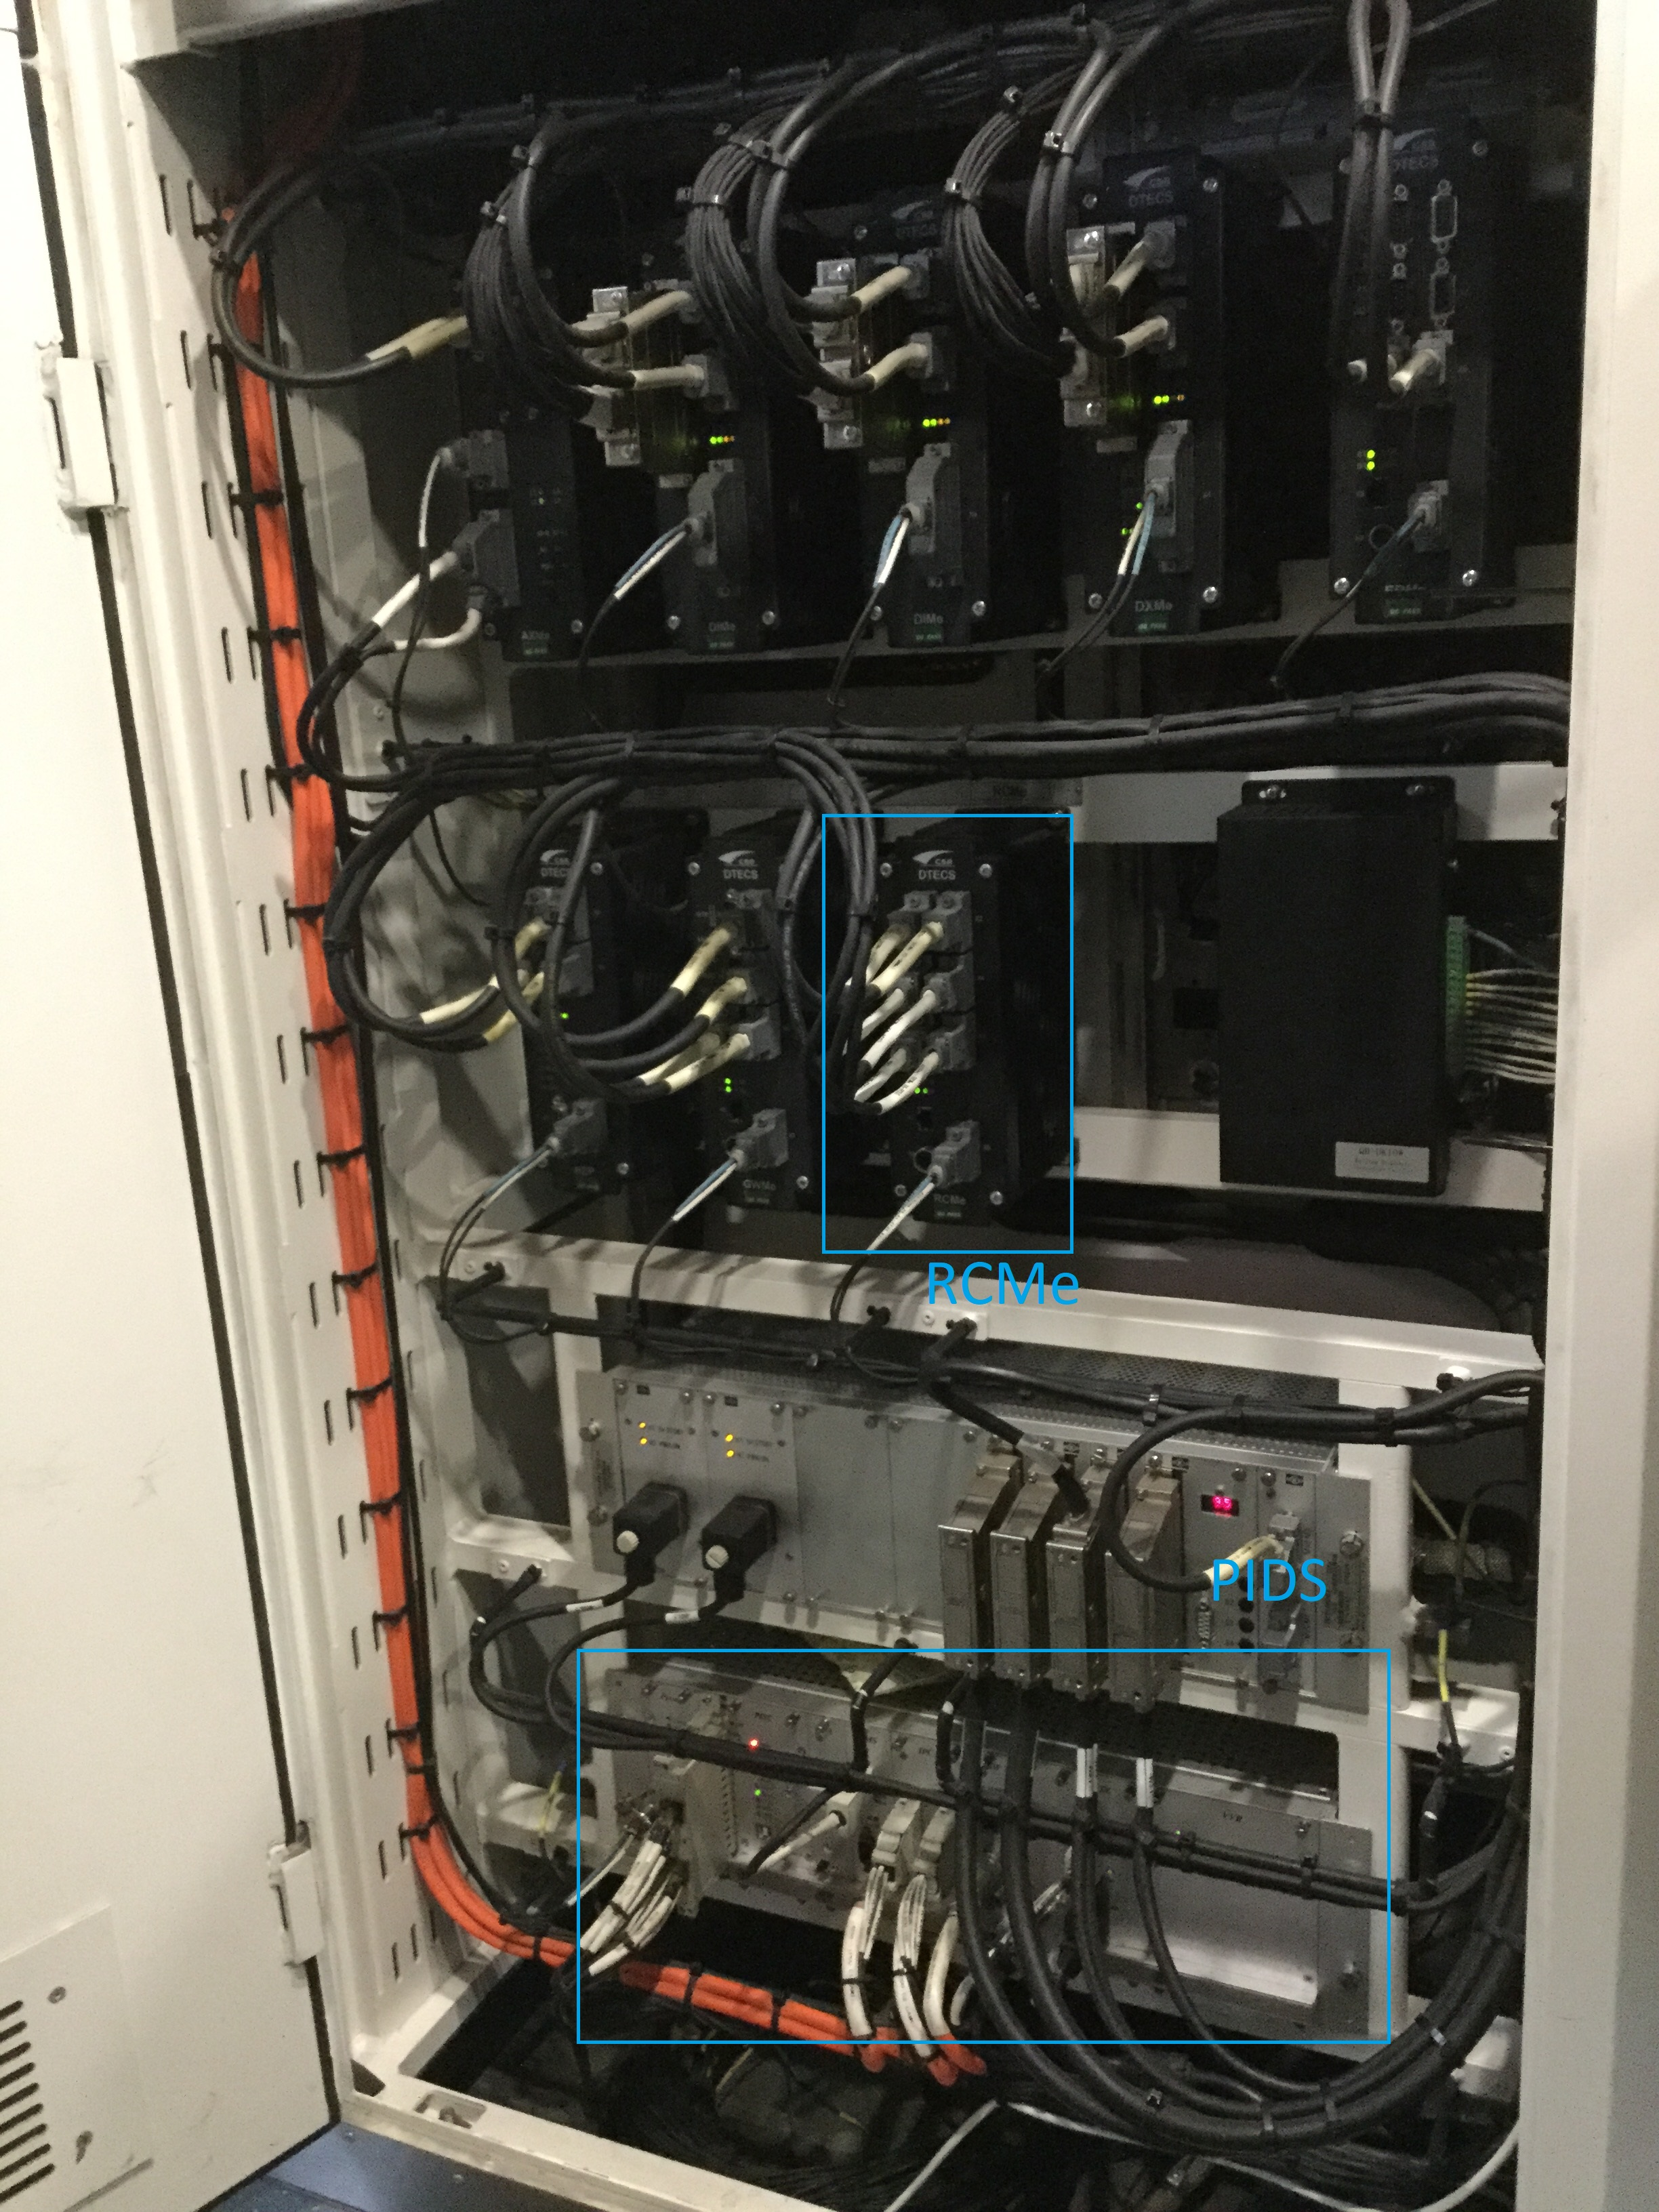
\includegraphics[width=1\textwidth , angle=90]{./Figures/imgRackTCN.JPG}
	\caption{}
	\label{fig:imgRackTCN}
\end{figure}



\pagebreak
\section{PIDS: Sistema de información visual para pasajeros de trenes}

\begin{figure}[ht]
	\centering
	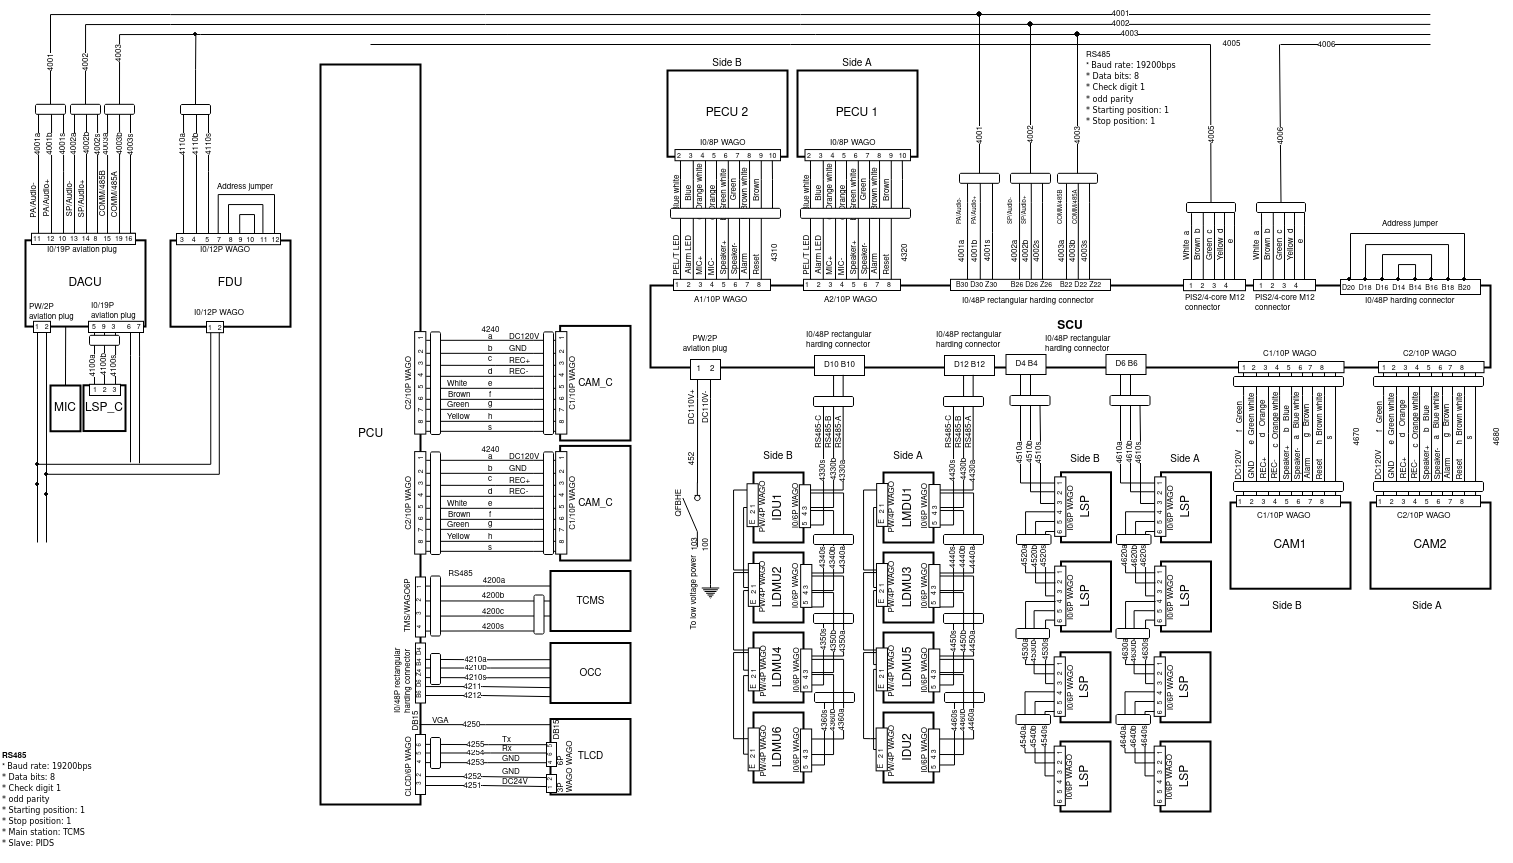
\includegraphics[width=1\textwidth , angle=90]{./Figures/diagramaPIDS.png}
	\caption{}
	\label{fig:diagramaPIDS}
\end{figure}


\begin{figure}[ht]
	\centering
	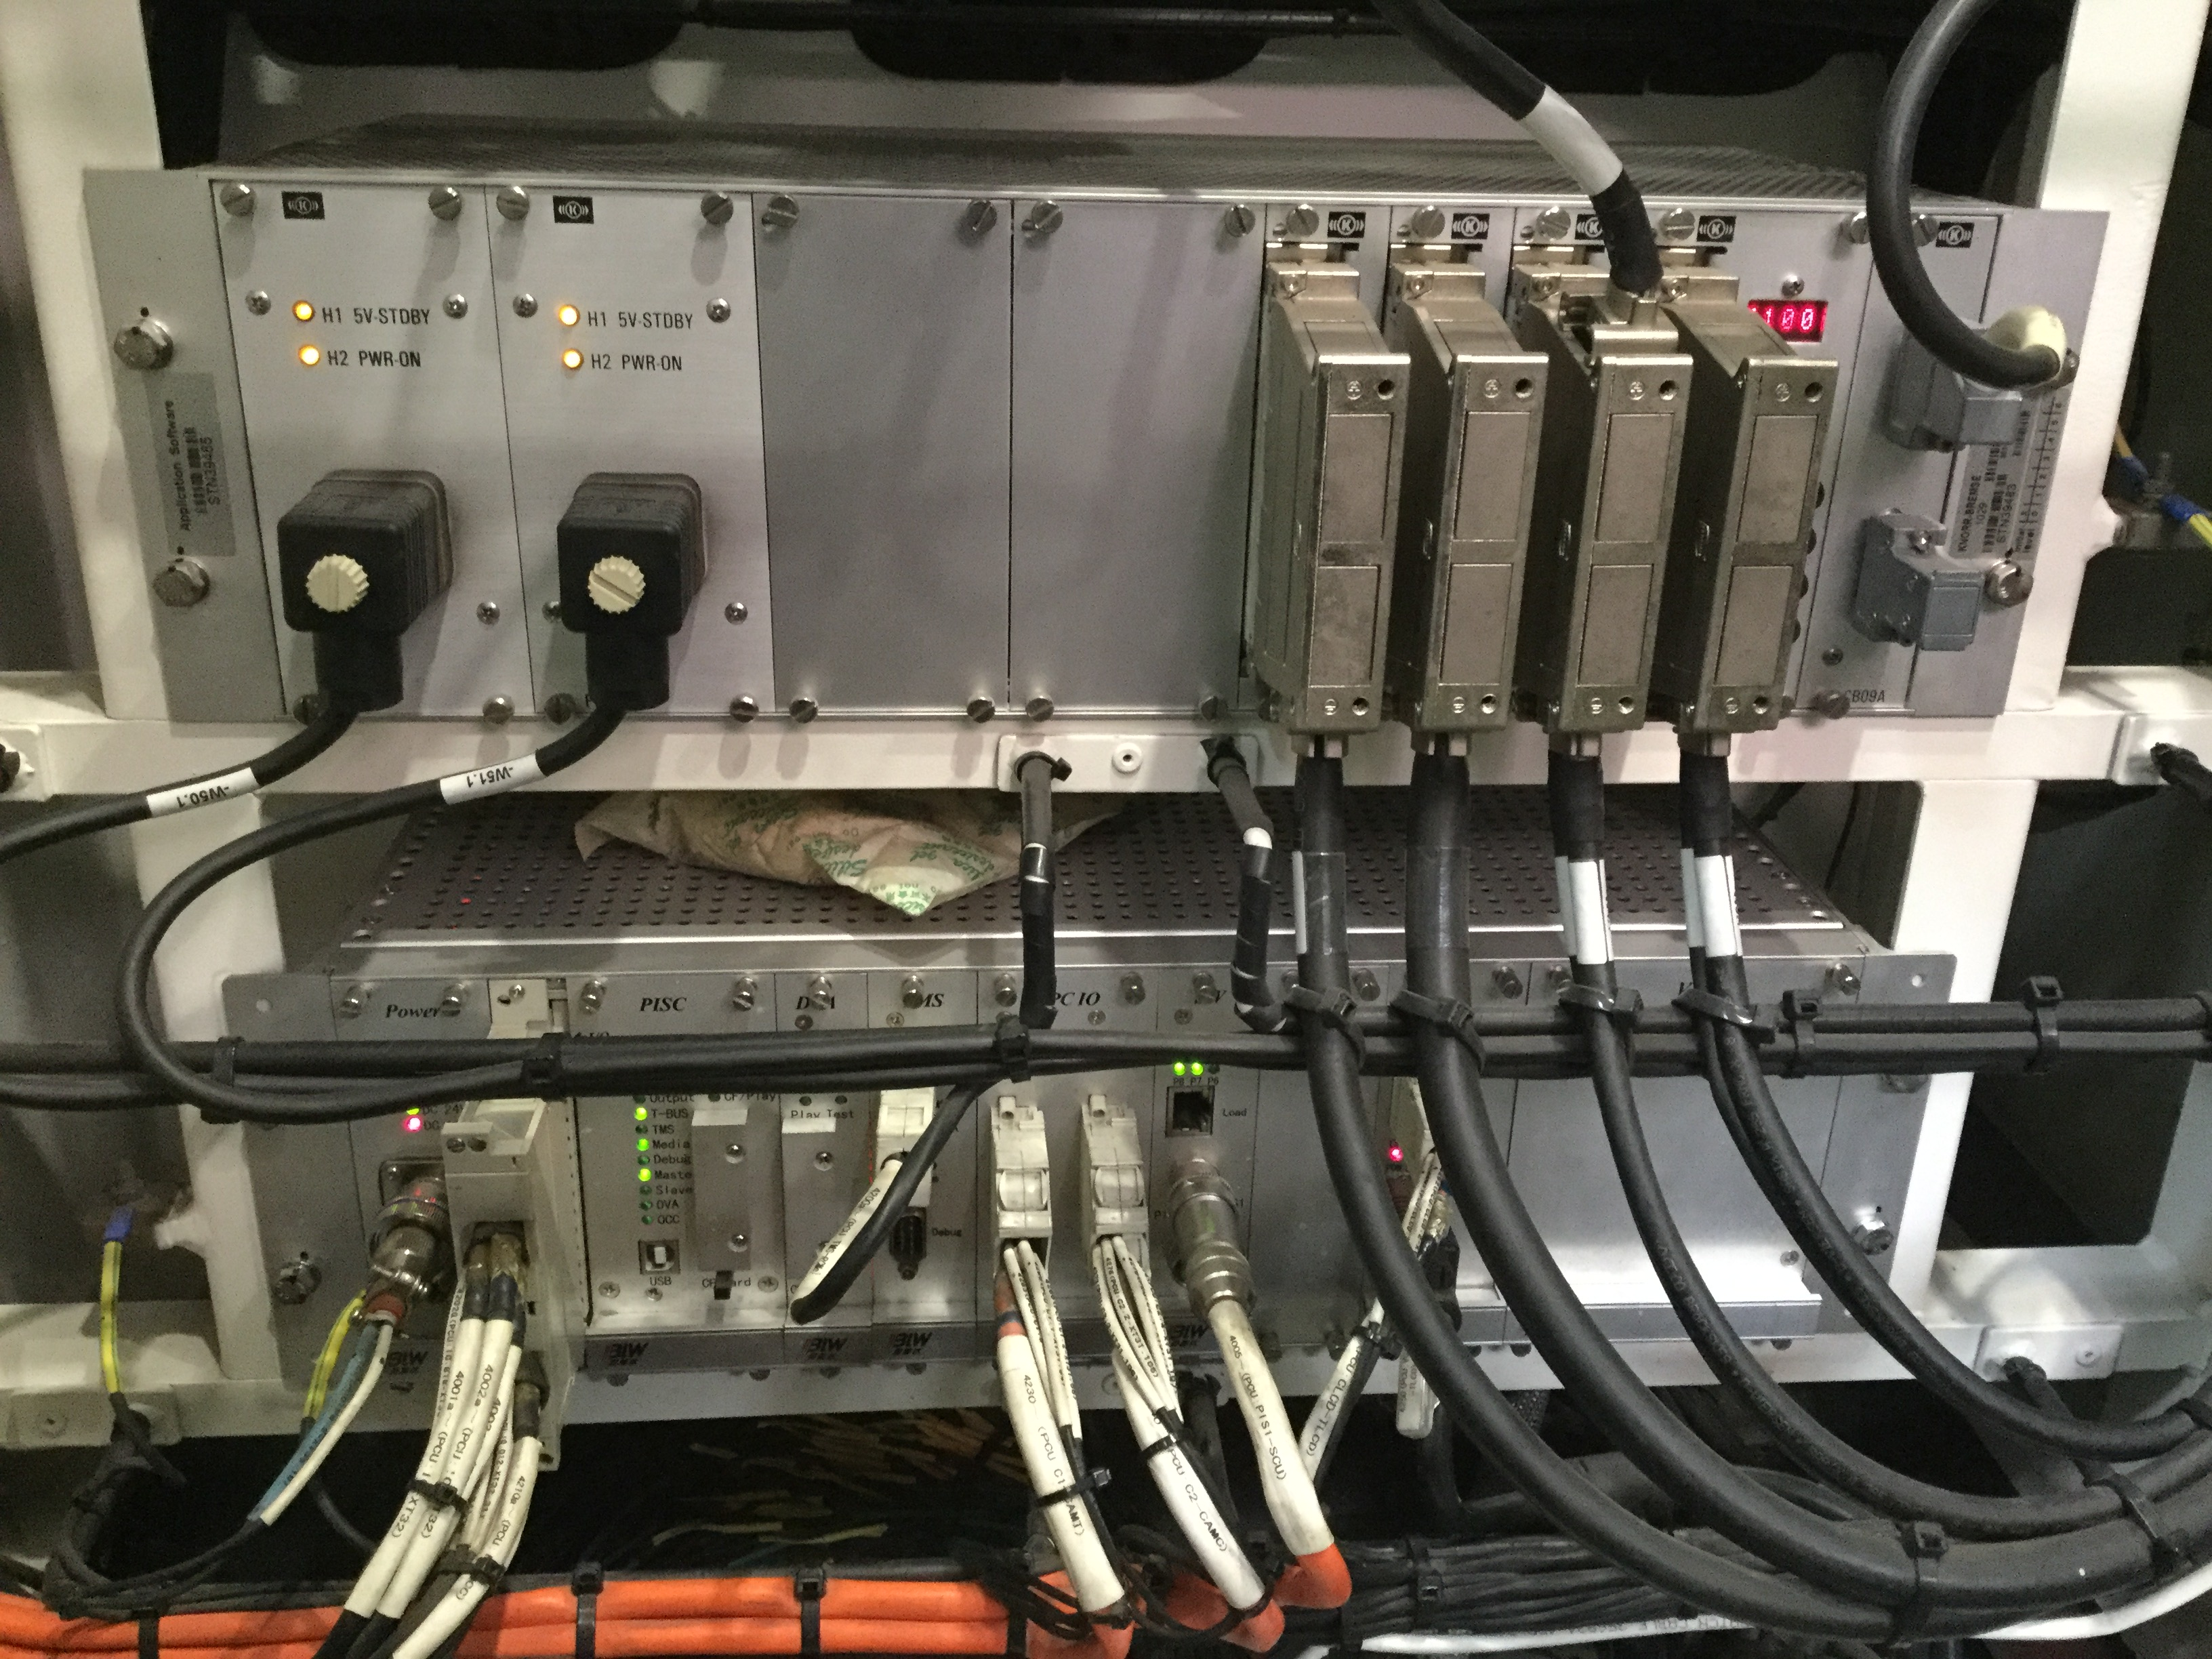
\includegraphics[width=1\textwidth]{./Figures/rackPIDS1.JPG}
	\caption{}
	\label{fig:rackPIDS1}
\end{figure}


\begin{figure}[ht]
	\centering
	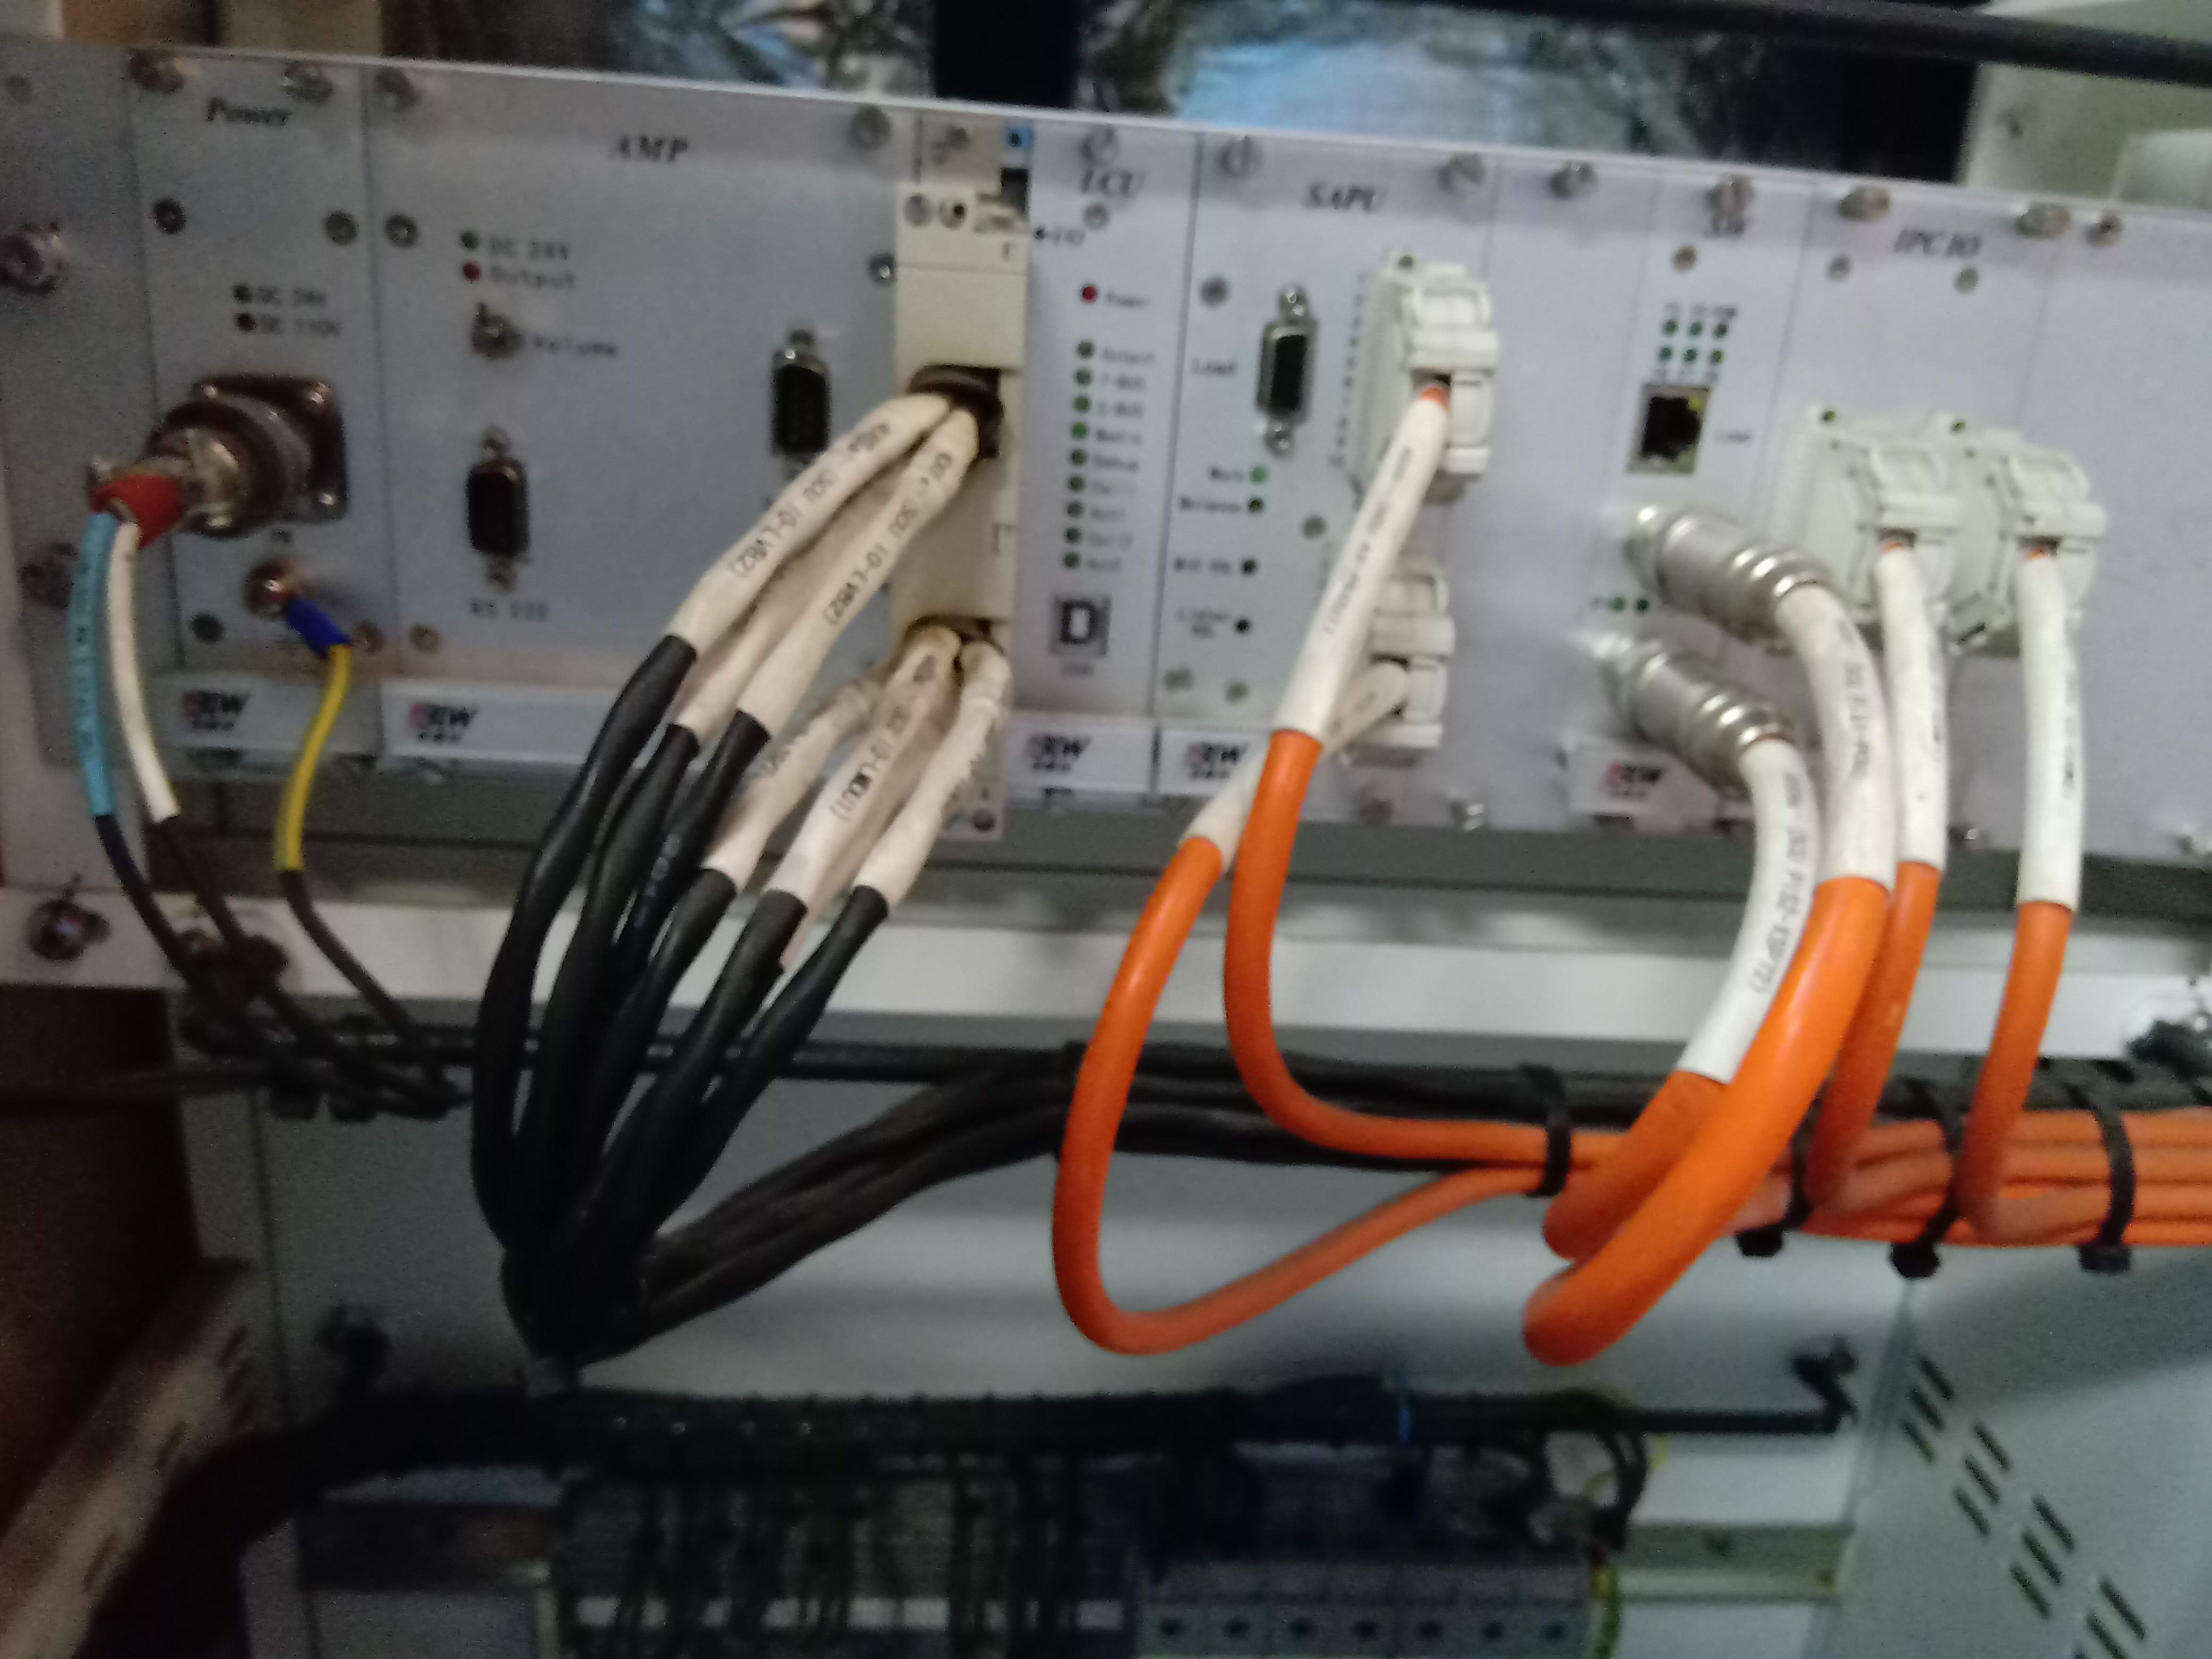
\includegraphics[width=1\textwidth ]{./Figures/rackPIDS2.jpg}
	\caption{}
	\label{fig:rackPIDS2}
\end{figure}


\pagebreak
\section{Carteles y controladoras de matrices LED}

\begin{figure}[ht]
	\centering
	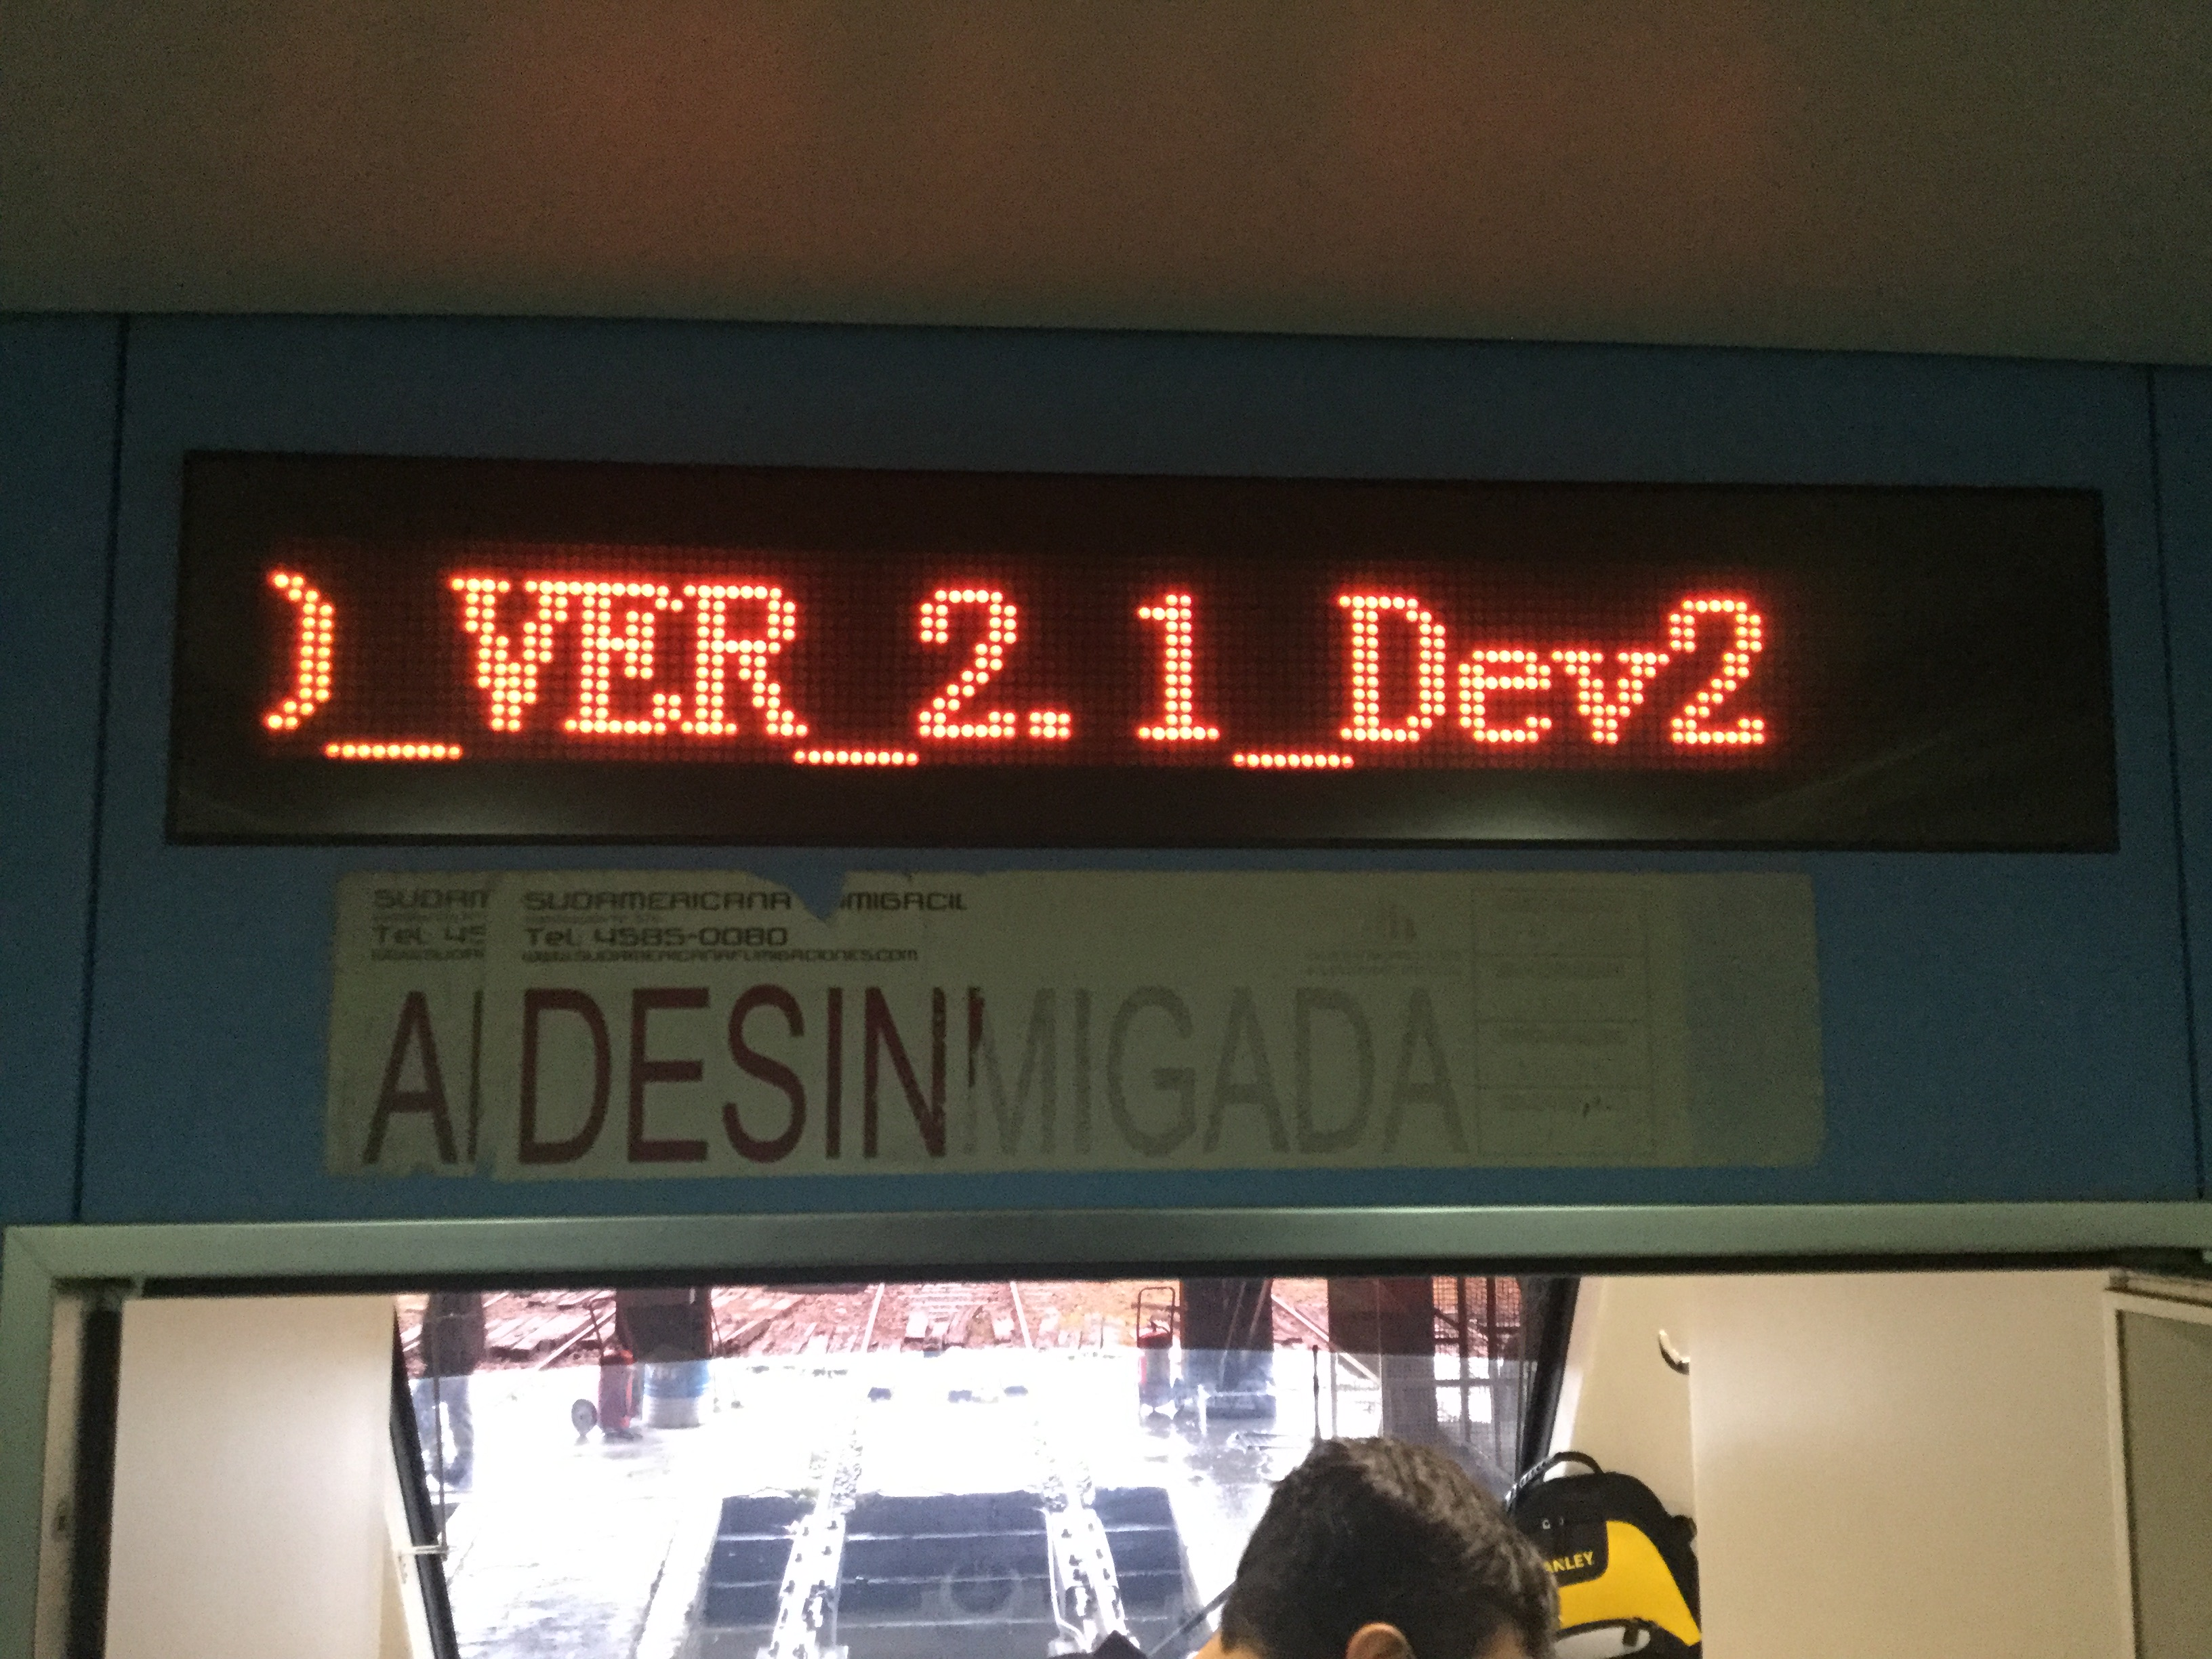
\includegraphics[width=1\textwidth]{./Figures/cartelIniciando.JPG}
	\caption{}
	\label{fig:cartelIniciando}
\end{figure}

\begin{figure}[ht]
	\centering
	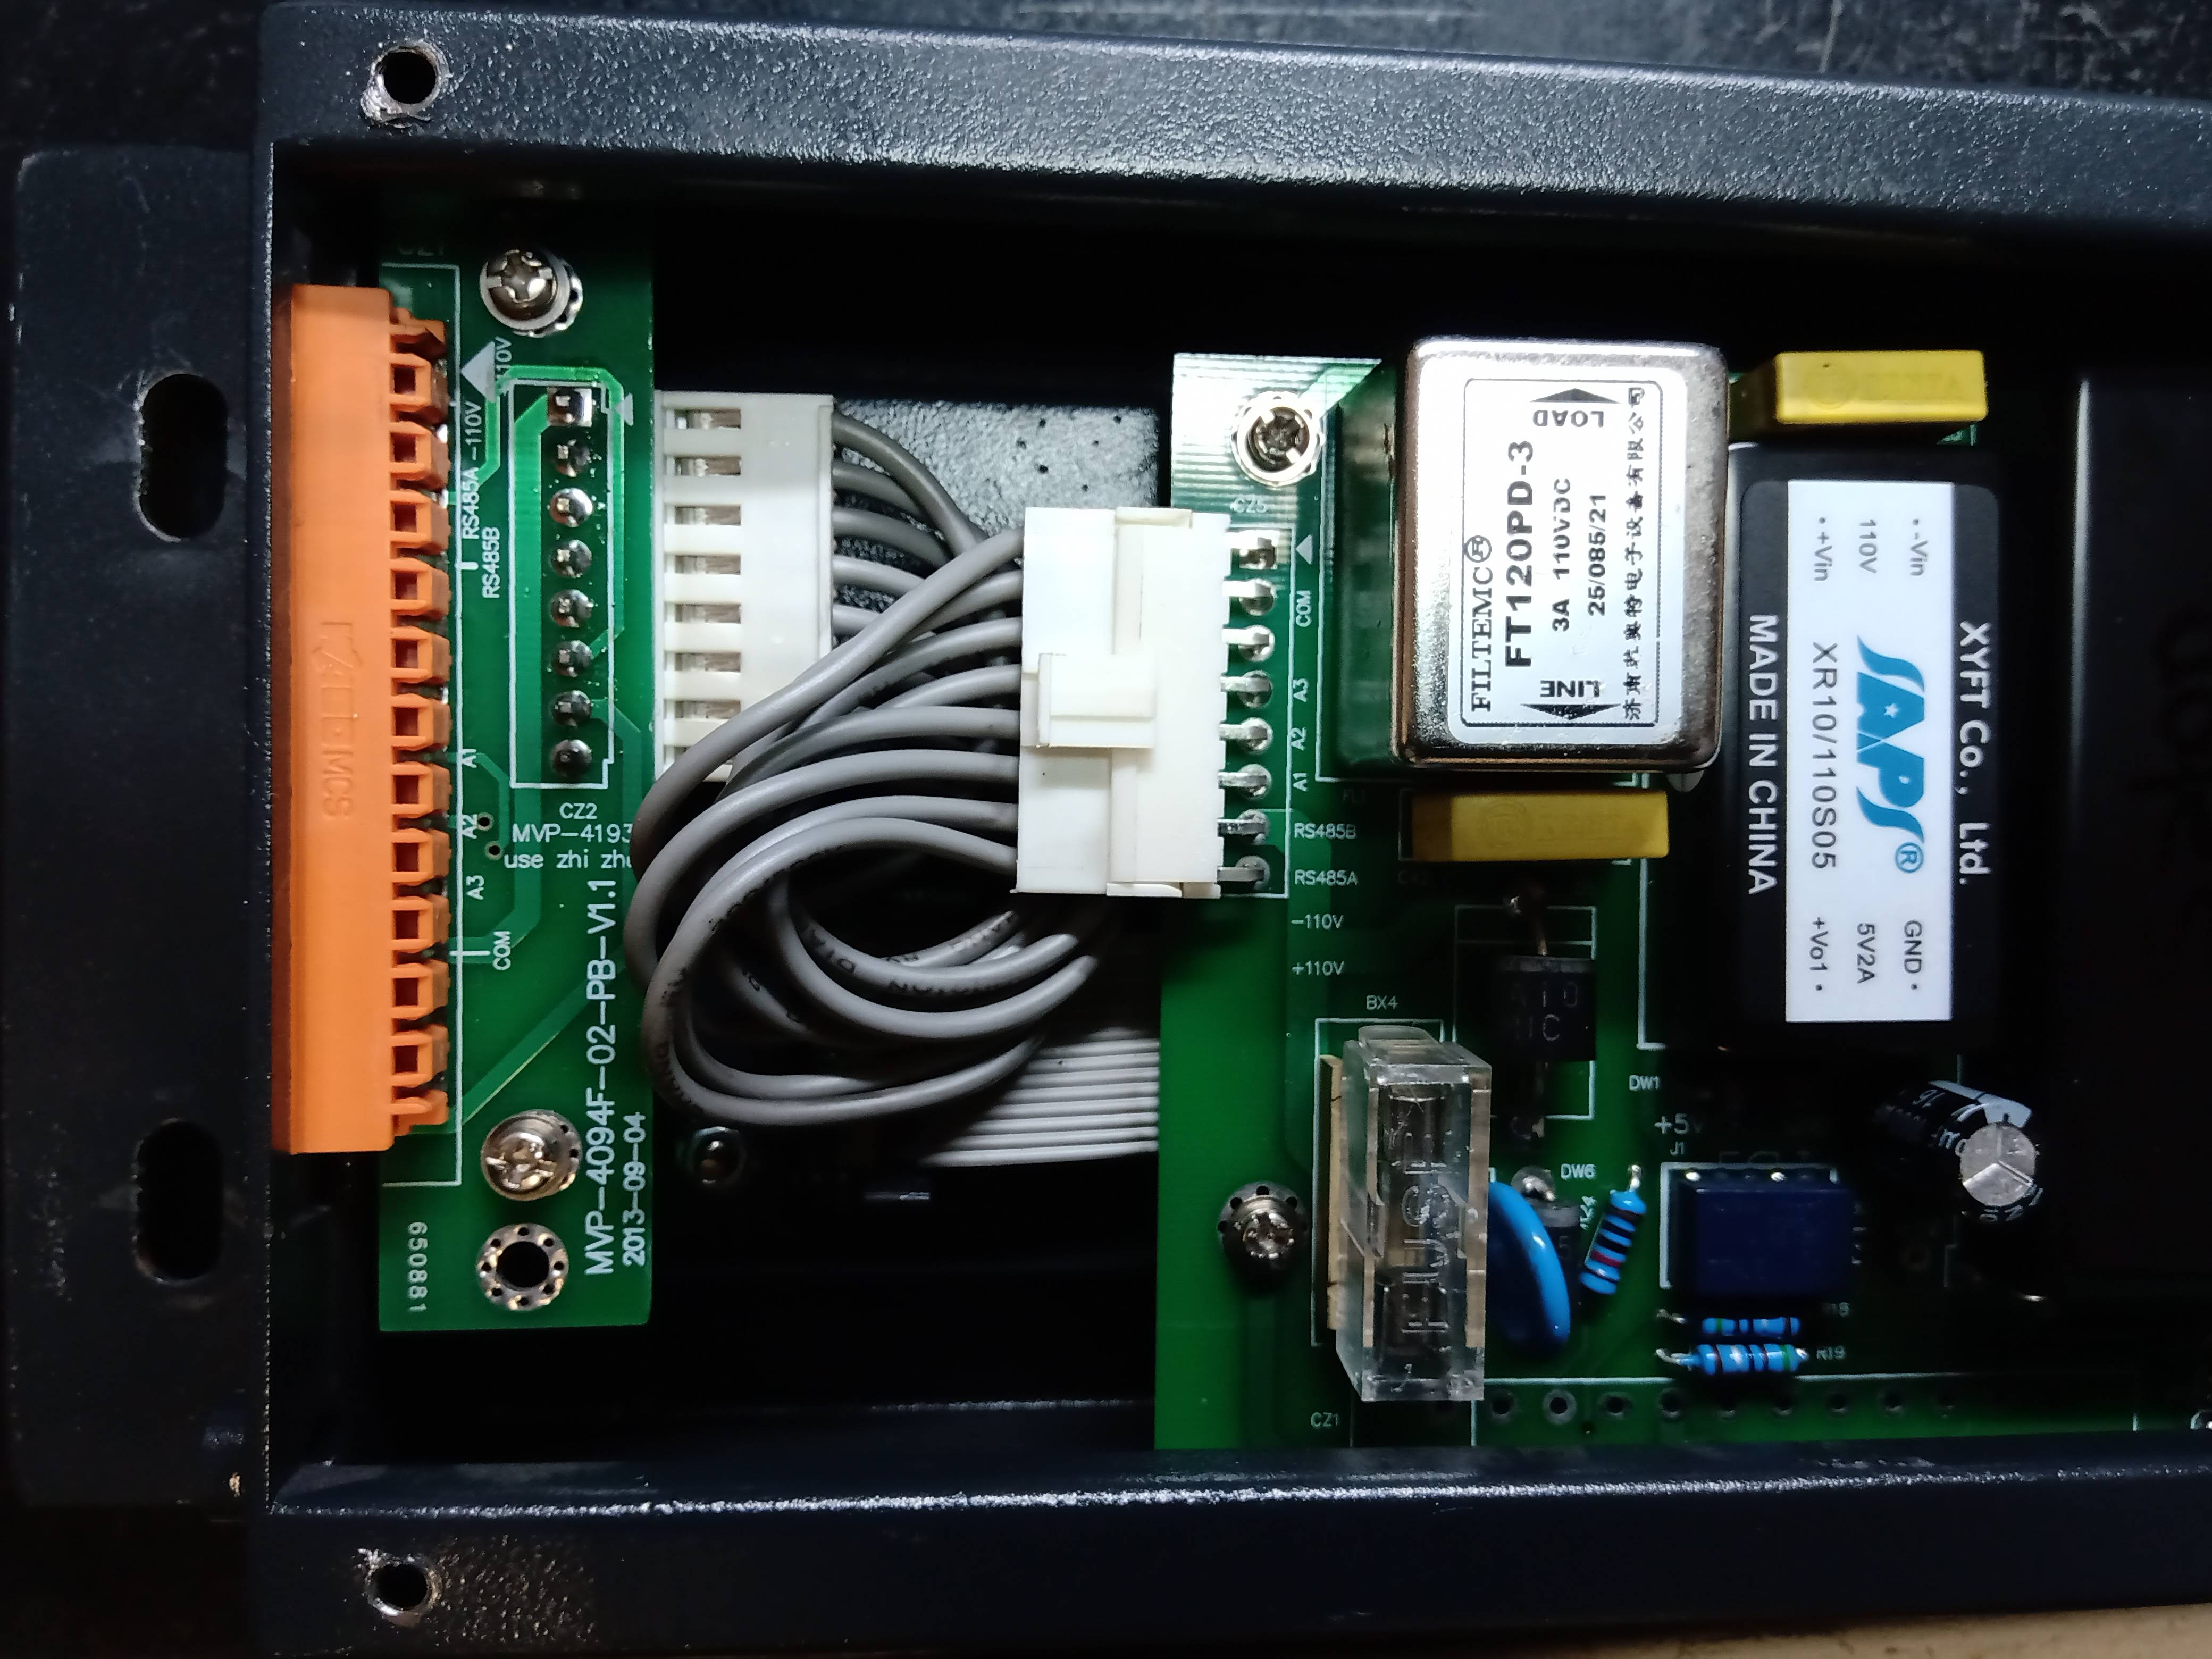
\includegraphics[width=1\textwidth]{./Figures/displayController.jpg}
	\caption{}
	\label{fig:displayController}
\end{figure}
